% !TEX root = ../main.tex

% Local fallback because the template does not define \mathscr.
\providecommand{\mathscr}[1]{\mathcal{#1}}

% ==================================================

\section{Methodology}
\label{sec:methodology}
% ==================================================

\subsection{Framework Overview and Problem Formulation}
\label{subsec:framework_formulation}

\HVM{} formulates edge--cloud VSLAM transmission as a VSLAM-oriented vision--language memory coding problem. Instead of sending a dense image stream to the cloud, the edge device selects sparse boundary frames and summarizes the omitted intervals with motion memory, semantic anchors, and language memory. The cloud then reconstructs task-usable intermediate views with a vision--language conditioned world-model decoder, and the resulting visual stream is consumed by a conventional cloud-side VSLAM estimator.

\begin{figure*}[!t]
\centering
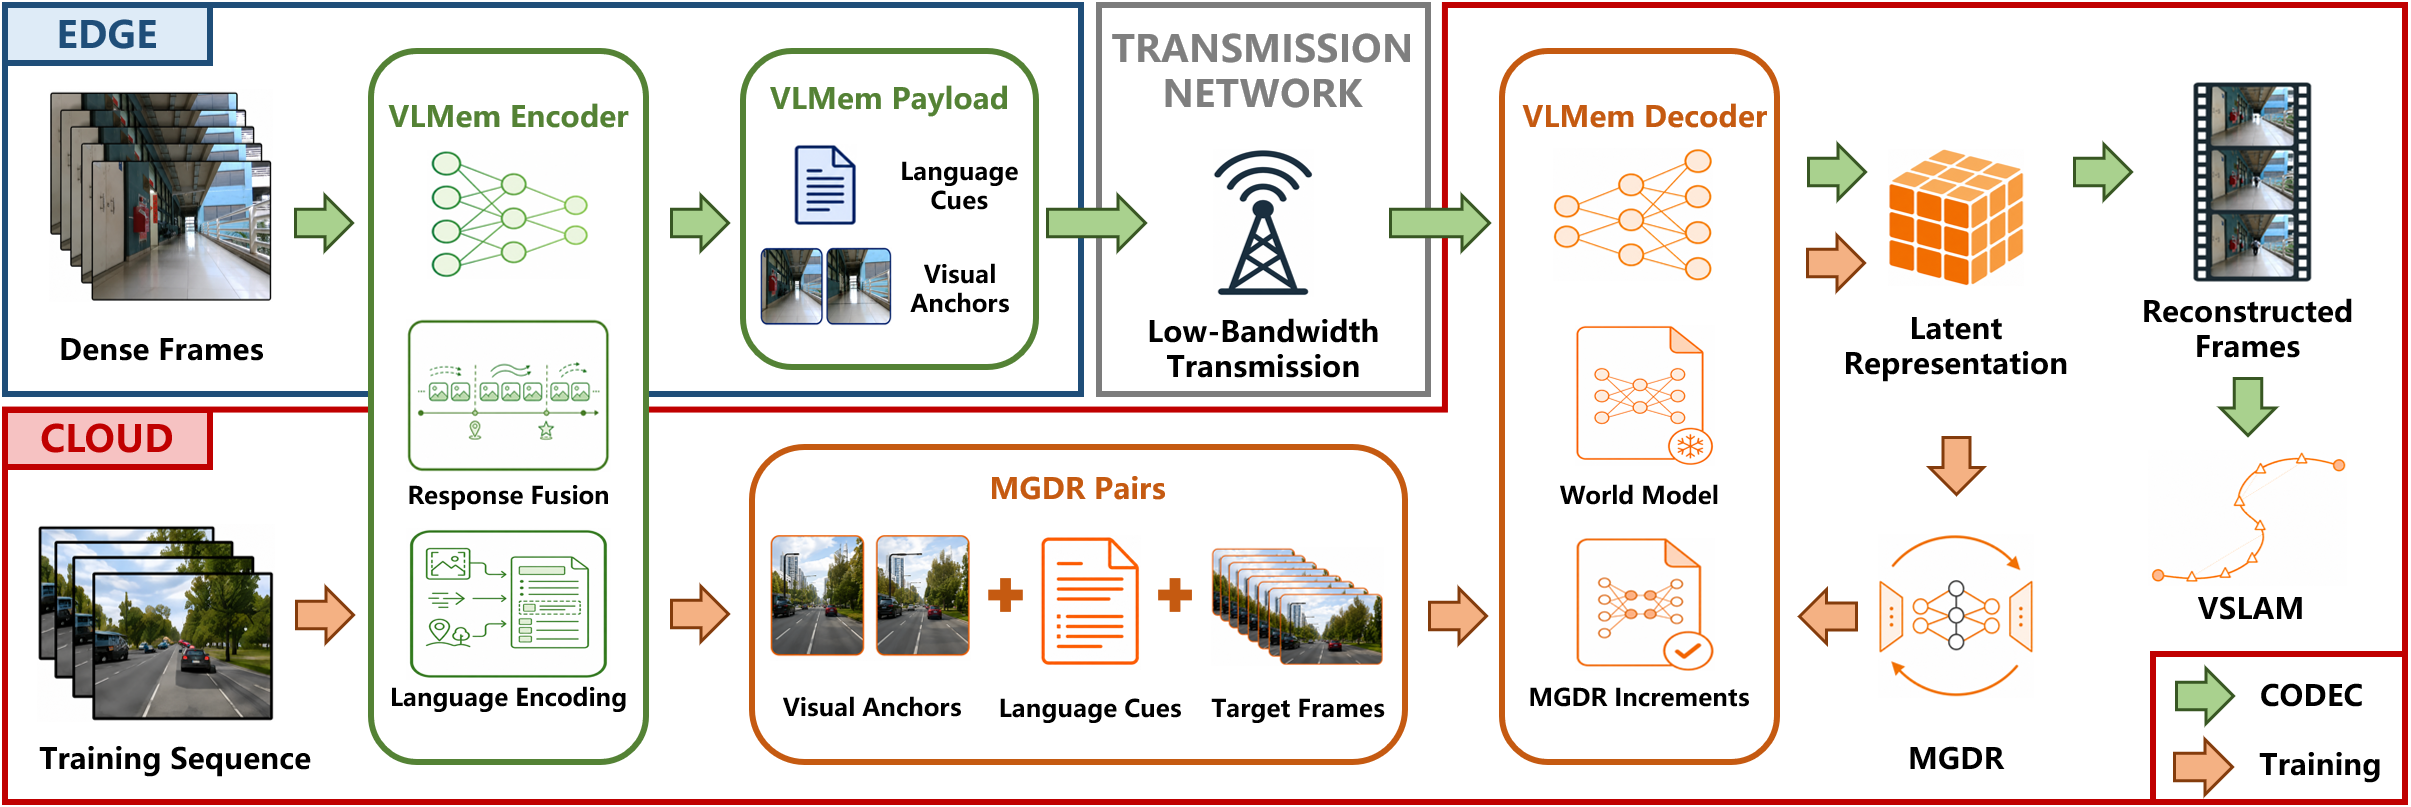
\includegraphics[width=\textwidth]{figures/fig2.png}
\caption{Overall framework of HVM-Codec for edge--cloud VSLAM visual transmission. The edge-side encoder converts dense visual streams into boundary frames, motion memory, semantic anchors, and compact language memory, while the cloud-side world-model decoder reconstructs task-usable visual sequences for downstream VSLAM. The same memory format is used for inference and memory-guided refinement.}
\label{fig:framework}
\end{figure*}

Fig.~\ref{fig:framework} gives the global pipeline. The edge device performs lightweight memory encoding over a fixed set of admissible temporal positions, transmits sparse vision--language memory, and leaves dense visual reconstruction to the cloud. The same memory format is used offline to prepare memory-guided refinement pairs, so the decoder observes consistent boundary-frame and language-memory conditions during refinement and inference.

Let the dense visual stream captured by the edge device be
\begin{equation}
\mathcal{I}_{1:T}
=\{I_t\}_{t=1}^{T},\qquad
I_t\in\mathbb{R}^{H\times W\times C}.
\label{eq:dense_stream}
\end{equation}
Here \(I_t\) is the \(t\)-th image in a sequence of length \(T\), and \(H\), \(W\), and \(C\) denote image height, width, and channels.

The edge encoder represents omitted intervals by vision--language memory units. Let \(\mathcal{P}\subseteq\{1,\ldots,T\}\) denote the admissible temporal positions from which boundaries and anchor candidates may be selected. Unit \(i\) is
\begin{equation}
\begin{aligned}
\mathcal{U}_i
=\big(&I_{b_i^-},I_{b_i^+},\mathcal{S}_i,\mathcal{A}_i,\\
&\mathcal{L}_i,\mathcal{L}_i^{-}\big),\qquad
b_i^-,b_i^+\in\mathcal{P}.
\end{aligned}
\label{eq:vl_memory_unit}
\end{equation}
The boundary frames \(I_{b_i^-}\) and \(I_{b_i^+}\) provide geometric and appearance constraints at the ends of the unit. The variable \(\mathcal{S}_i\) is motion memory, \(\mathcal{A}_i\) is the set of semantic anchors, and \(\mathcal{L}_i\) and \(\mathcal{L}_i^{-}\) are positive and negative language memory.

The edge-side memory encoder \(\mathcal{E}_{\phi}\) and cloud-side world-model decoder \(\mathcal{G}_{\theta+\Delta\theta}\) are written compactly as
\begin{equation}
\begin{aligned}
\mathcal{M}
&=\mathcal{E}_{\phi}(\mathcal{I}_{1:T};\mathcal{P})
=\{\mathcal{U}_i\}_{i=1}^{N},\\
\widehat{\mathcal{I}}_{1:T}
&=\mathcal{G}_{\theta+\Delta\theta}(\mathcal{M}).
\end{aligned}
\label{eq:memory_coding}
\end{equation}
The memory \(\mathcal{M}\) is not a conventional pixel bitstream. It is sparse vision--language memory containing boundary frames, motion memory, semantic-anchor indicators, language memory, and metadata needed for task-usable visual reconstruction on the cloud side. The increment \(\Delta\theta\) denotes optional decoder refinement increments applied to the pretrained decoder; Sec.~\ref{subsec:wm_lora_decoding} instantiates these increments with LoRA. With \(\Delta\theta=0\), the same notation describes the original unrefined world-model decoder. The small constant \(\epsilon\) used in later normalized ratios is introduced only for stable normalization.

Let \(\mathcal{B}\) denote the boundary positions and let \(\mathcal{K}=\{I_b\mid b\in\mathcal{B}\}\) be the transmitted boundary-frame set. The transmission cost is
\begin{equation}
\begin{aligned}
\mathcal{R}(\mathcal{M})
=&\mathcal{R}(\mathcal{K})
+\sum_{i=1}^{N}
\mathcal{R}(\mathcal{S}_i,\mathcal{A}_i,\mathcal{L}_i,\mathcal{L}_i^{-})\\
&+\mathcal{R}(\mathrm{meta}),\qquad
\mathcal{K}=\{I_b\mid b\in\mathcal{B}\}.
\end{aligned}
\label{eq:transmission_cost}
\end{equation}
Here \(\mathcal{R}(\cdot)\) denotes payload size. The compact memory term covers motion memory, semantic-anchor indicators, and language memory; Eq.~\eqref{eq:transmission_cost} is a rate model for reasoning about payload, not a claim that all components contribute equally.

The VSLAM-oriented rate--trajectory design criterion is
\begin{equation}
\begin{aligned}
\mathcal{M}^{\star}
=\arg\min_{\mathcal{M}\in\Omega}\;
&\mathcal{R}(\mathcal{M})\\
&+\lambda\mathcal{D}_{\mathrm{slam}}\!\left(
\mathcal{F}_{\mathrm{slam}}(\widehat{\mathcal{I}}_{1:T}),
\mathcal{T}\right).
\end{aligned}
\label{eq:rate_trajectory_design}
\end{equation}
Here \(\Omega\) is the admissible family of memory representations, \(\lambda\) is the trade-off coefficient between transmission cost and downstream trajectory discrepancy, \(\mathcal{F}_{\mathrm{slam}}\) is the cloud-side VSLAM estimator, \(\mathcal{T}\) is the reference trajectory when available, and \(\mathcal{D}_{\mathrm{slam}}\) is evaluated through APE RMSE in the experiments.

Eq.~\eqref{eq:rate_trajectory_design} is a VSLAM-oriented rate--trajectory design criterion rather than a closed-form optimization solved by the implementation. Conventional rate--distortion coding usually measures pixel distortion or perceptual reconstruction error. HVM-Codec instead treats task distortion as downstream VSLAM trajectory quality after task-usable visual reconstruction. In this paper, the two sides of the criterion are evaluated empirically through payload size and APE RMSE, while auxiliary image-fidelity metrics are reported separately.

\subsection{Motion--Semantic Event Memory Encoding}
\label{subsec:motion_semantic_segmentation}

The edge encoder constructs memory units from two complementary cues: a block-wise motion trend response and a semantic-anchor response. The motion trend response identifies forward motion, turning, and mixed transitions that affect viewpoint continuity. Semantic anchors capture embedding-level scene/content changes that should constrain admissible unit spans even when the coarse motion regime remains stable.

\begin{figure*}[!t]
\centering
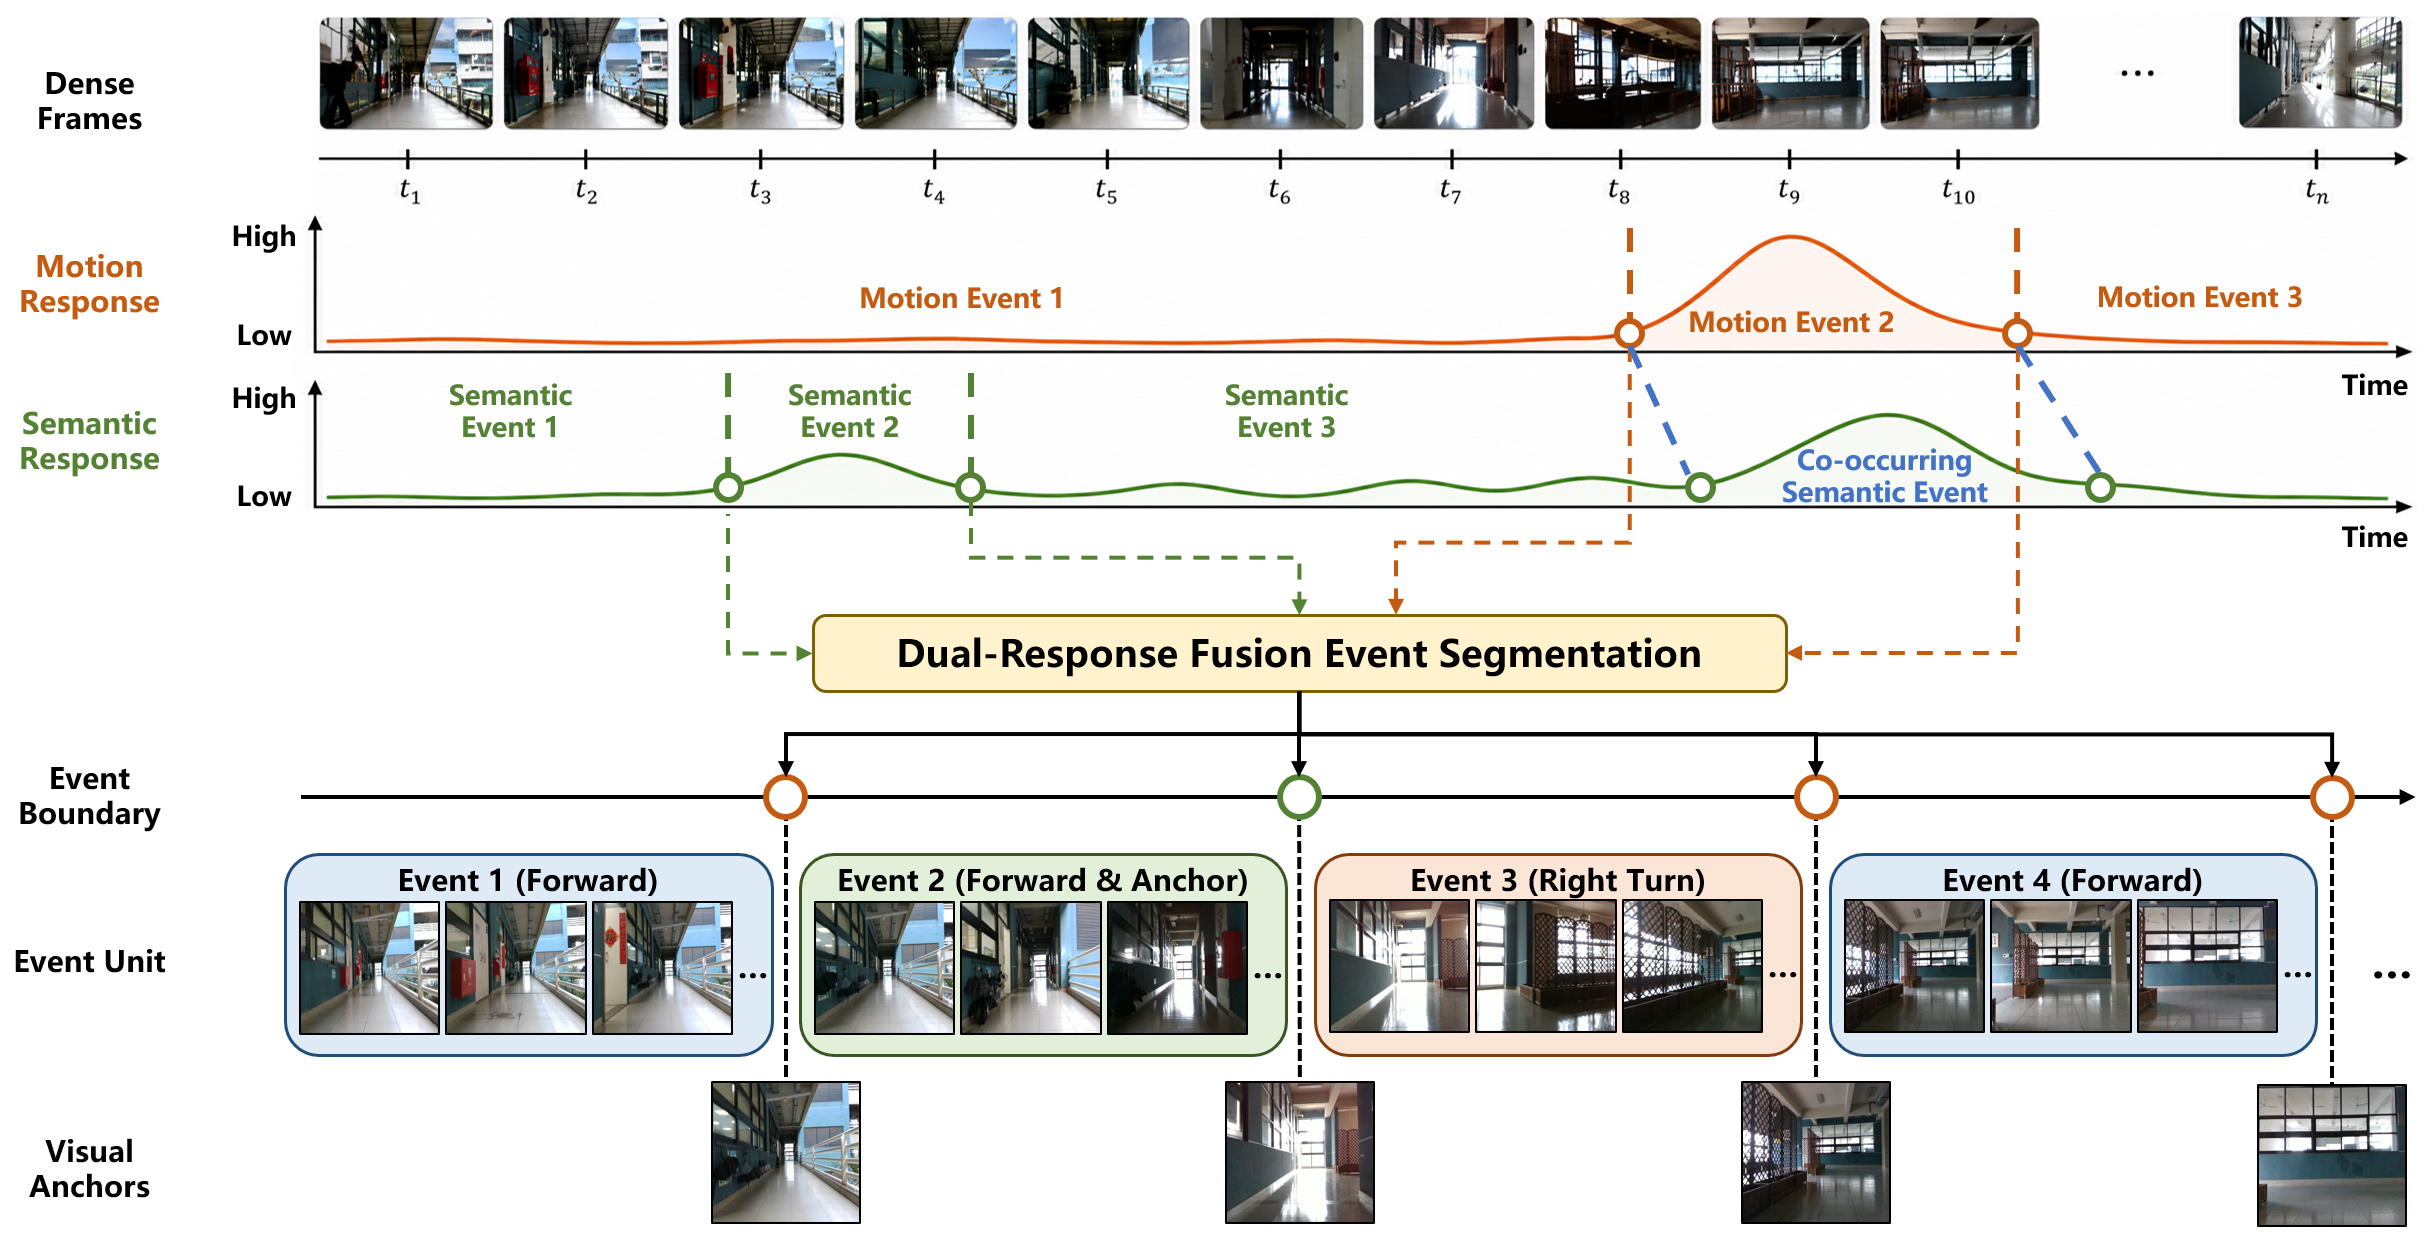
\includegraphics[width=0.92\textwidth]{figures/fig3.png}
\caption{Motion--semantic response fusion. Motion trend responses and semantic anchor responses are fused to divide the dense visual stream into vision--language memory units. Each unit is represented by boundary frames, motion memory, semantic anchors, and compact language memory.}
\label{fig:event_segmentation}
\end{figure*}

As shown in Fig.~\ref{fig:event_segmentation}, the encoder estimates low-cost motion trend response between consecutive frames by block-wise phase correlation. The encoder does not require dense pixel-level correspondence; it needs motion-regime-level evidence for boundary construction and motion-conditioned language memory. Each frame is divided into spatial blocks indexed by \(g\), \(I_t^g\) denotes the corresponding image patch, and \(H\) is a local windowing mask. The phase-correlation response is
\begin{equation}
\begin{aligned}
\widetilde{I}_{t}^{g}
&=H\odot I_t^g,\\
\mathcal{C}_{t,g}
&=\mathscr{F}^{-1}\!\left(
\frac{
\mathscr{F}(\widetilde{I}_{t}^{g})
\mathscr{F}(\widetilde{I}_{t-1}^{g})^{*}}
{\left|
\mathscr{F}(\widetilde{I}_{t}^{g})
\mathscr{F}(\widetilde{I}_{t-1}^{g})^{*}
\right|+\epsilon}\right),\\
(\mathbf{d}_{t,g},\rho_{t,g})
&=\operatorname{Peak}(\mathcal{C}_{t,g}).
\end{aligned}
\label{eq:block_phase_correlation}
\end{equation}
Here \(\odot\) denotes element-wise multiplication, \(\mathscr{F}\) is the Fourier transform, \((\cdot)^{*}\) is complex conjugation, \(\mathbf{d}_{t,g}\) is the block displacement, and \(\rho_{t,g}\) is the peak confidence. The block-wise form provides a lightweight trend cue without dense optical flow. Because each block contributes a local displacement peak, the following aggregation can capture coarse camera behavior while staying inexpensive enough for edge-side memory encoding.

The encoder downweights blocks whose phase-correlation peaks or visual texture are unreliable. This is summarized by the reliability function
\begin{equation}
w_{t,g}
=\omega_{\mathrm{rel}}
\left(
\rho_{t,g},
\sigma(I_{t-1}^{g}),
g
\right).
\label{eq:block_reliability}
\end{equation}
The function \(\omega_{\mathrm{rel}}\) combines peak confidence, local texture strength \(\sigma(I_{t-1}^{g})\), and row-position reliability. It suppresses weakly textured or unreliable blocks before the motion descriptors are accumulated. This reliability weighting is important because texture-poor regions and unstable block peaks can otherwise dominate a simple average and create spurious motion-regime changes.

The weighted block displacements define two compact motion descriptors:
\begin{equation}
\begin{aligned}
\bar{\mathbf{d}}_{t}
&=
\frac{\sum_g w_{t,g}\mathbf{d}_{t,g}}
{\sum_g w_{t,g}+\epsilon},\\
\chi_t
&=
\frac{\sum_g w_{t,g}
\left(x'_g d^{x}_{t,g}+y'_g d^{y}_{t,g}\right)}
{\sum_g w_{t,g}\left((x'_g)^2+(y'_g)^2\right)+\epsilon}.
\end{aligned}
\label{eq:motion_descriptors}
\end{equation}
Here \(\bar{\mathbf{d}}_t\) is the reliability-weighted global displacement trend, \(\chi_t\) is radial expansion evidence related to forward motion, and \((x'_g,y'_g)\) are normalized block-center coordinates.

The descriptors are converted into motion trend scores and a coarse motion regime. Let \(\zeta_t\) denote the yaw-like lateral response derived from the reliability-weighted block displacement field:
\begin{equation}
\begin{aligned}
r_t^{\mathrm{turn}}
&=\frac{|\zeta_t|}{s_m+\epsilon}c_t^{\mathrm{sgn}},
\qquad
r_t^{\mathrm{fwd}}
=\frac{\max(\chi_t,0)}{s_m+\epsilon}c_t^{\mathrm{exp}},\\
s_t
&=\Gamma_m(r_t^{\mathrm{turn}},
r_t^{\mathrm{fwd}},c_t^{\mathrm{sgn}}),
\qquad
s_t\in\mathcal{S}_{\mathrm{motion}}.
\end{aligned}
\label{eq:motion_regime_assignment}
\end{equation}
The scalar \(s_m\) normalizes the motion scale, \(c_t^{\mathrm{sgn}}\) measures left/right sign consistency, and \(c_t^{\mathrm{exp}}\) measures expansion consistency. The rule \(\Gamma_m\) is a lightweight mapping from motion trend scores to coarse motion regimes such as forward, left-turn, right-turn, and mixed; it is not a learned classifier.

Frame-level regimes are stabilized over admissible temporal windows:
\begin{equation}
\begin{aligned}
\ell_j
&=\Gamma_w(\{s_t,r_t^{\mathrm{turn}},
r_t^{\mathrm{fwd}},\rho_t\}_{t\in W_j}),\\
\widetilde{\ell}_j
&=\operatorname{Stab}_{\tau_\rho}
(\ell_{j-1},\ell_j,\ell_{j+1},\bar{\rho}_j).
\end{aligned}
\label{eq:window_stabilization}
\end{equation}
Here \(W_j\) is an admissible temporal window, \(\rho_t\) is frame-level confidence aggregated from block responses, and \(\bar{\rho}_j\) is the window-average confidence. The label \(\ell_j\) is the window-level motion regime, while \(\widetilde{\ell}_j\) suppresses isolated low-confidence regime changes when neighboring windows agree. This stabilization is needed because frame-level motion evidence can be noisy, especially near weak texture or transient viewpoint changes. By preserving persistent transitions while suppressing unreliable one-window changes, it reduces unnecessary fragmentation of the memory representation.

Semantic anchors complement motion memory by detecting embedding-level scene/content changes. For a candidate admissible position \(p\) and current semantic context \(c\), define
\begin{equation}
\begin{aligned}
\mathbf{z}_{p}
&=\frac{f_{\psi}(I_p)}{\|f_{\psi}(I_p)\|_2},
\qquad
r_p^{\mathrm{sem}}(c)=1-\mathbf{z}_{p}^{\top}\mathbf{z}_{c},\\
\mathcal{A}
&=\Big\{a\in\mathcal{P}\ \Big|
\operatorname{Pers}_{P_{\min}}
\big(r_a^{\mathrm{sem}}(c)>\tau_a(s)\big),\\
&\qquad\qquad
\operatorname{Sep}(a;c,b^+)\ge g_{\min}\Big\}.
\end{aligned}
\label{eq:semantic_anchor_admission}
\end{equation}
Here \(f_{\psi}\) is the image embedding encoder, \(\mathbf{z}_{p}\) and \(\mathbf{z}_{c}\) are normalized embeddings, and \(r_p^{\mathrm{sem}}(c)\) is the semantic-anchor response relative to the current semantic context \(c\). The context \(c\) need not be the immediately preceding frame; it represents the active scene/content reference used for the current interval. The operator \(\operatorname{Pers}_{P_{\min}}\) requires enough supporting admissible positions, and \(\operatorname{Sep}\) enforces separation from the semantic context and the unit boundary. The threshold \(\tau_a(s)\) depends on the motion regime \(s\), and \(\mathrm{turn}\) denotes either left-turn or right-turn regimes. Semantic anchors are embedding-level scene/content changes rather than hand-labeled object categories.

Finally, semantic anchors and admissible unit spans are combined through sequential boundary construction. Let \(\Delta_s\) be the motion-regime-dependent admissible unit span set and \(e\) the endpoint of the current interval:
\begin{equation}
\begin{aligned}
\mathcal{N}_k
&=\{p\in\mathcal{P}\mid b_k<p\le e,\;
p-b_k\in\Delta_s,\\
&\qquad\operatorname{Reach}(p,e;\Delta_s)=1\},\\
b_{k+1}
&=
\begin{cases}
\min(\mathcal{N}_k\cap\mathcal{A}),
& \mathcal{N}_k\cap\mathcal{A}\neq\varnothing,\\
\max\mathcal{N}_k, & \mathrm{otherwise}.
\end{cases}
\end{aligned}
\label{eq:admissible_boundary_construction}
\end{equation}
Here \(\mathcal{N}_k\) is the set of admissible next boundary positions from the current boundary \(b_k\), and \(\operatorname{Reach}(p,e;\Delta_s)\) ensures that the remaining interval can still be covered by valid spans. The construction chooses the earliest admissible semantic anchor when one is available; otherwise, it advances to the farthest reachable admissible boundary. This is a sequential construction, not a global optimization.

The complete event-memory encoding in III-B therefore has three stages. Block-wise phase correlation provides a low-cost motion trend response, semantic-anchor response adds embedding-level scene/content-change constraints, and admissible boundary construction combines both cues into vision--language memory units. The two responses are complementary: motion cues shorten difficult turn and mixed intervals where viewpoint change is harder to reconstruct, while semantic anchors prevent long stable-motion intervals from becoming visually underconstrained.

\subsection{Dual-Branch World-Model Decoding}
\label{subsec:wm_lora_decoding}

The cloud-side decoder has two coupled branches. The inference branch reconstructs task-usable intermediate frames from the transmitted vision--language memory, while the refinement branch performs \emph{memory-guided world-model refinement}. This refinement uses the same memory format as inference, exposing the decoder during refinement to the same type of boundary frames and language memory that it receives during deployment.

\begin{figure}[!t]
\centering
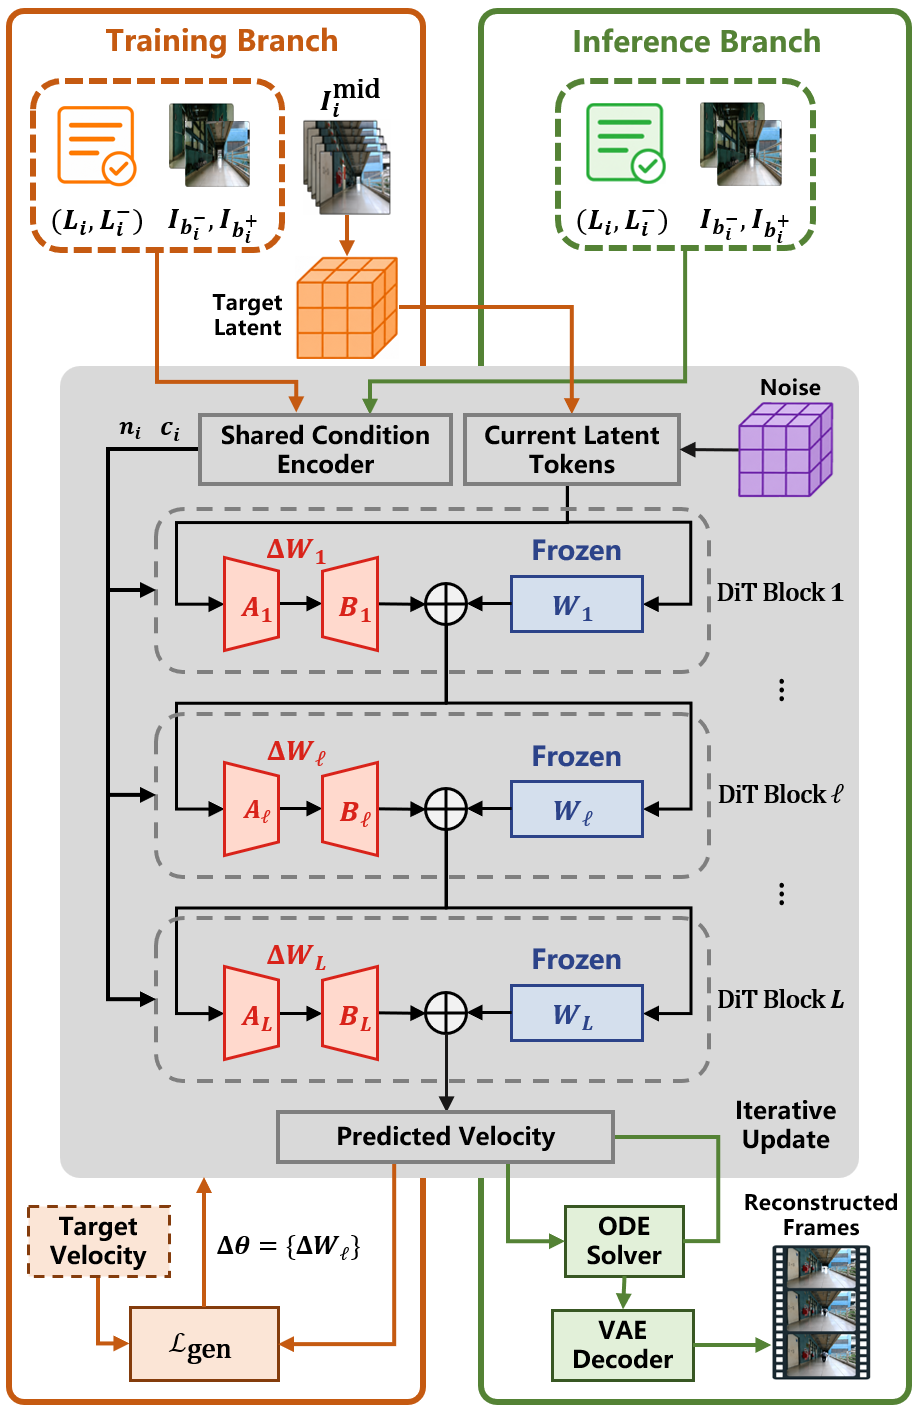
\includegraphics[width=0.95\columnwidth]{figures/fig4.png}
\caption{Dual-branch world-model decoding. The inference branch reconstructs intermediate frames from transmitted boundary frames and language memory. The refinement branch uses the same memory format to construct LoRA-based refinement pairs while keeping the pretrained world model frozen.}
\label{fig:lora_decoder}
\end{figure}

Fig.~\ref{fig:lora_decoder} illustrates the two branches. Boundary frames provide visual constraints that language memory cannot precisely express, while language memory supplies compact motion-conditioned priors for the omitted interval. First, each unit forms language memory from the shared navigation prior and the motion regime:
\begin{equation}
\begin{aligned}
\mathcal{L}_i
&=\operatorname{Join}\left(
\mathcal{L}_{\mathrm{base}},
\mathcal{L}_{\mathrm{motion}}(s_i)\right),\\
\mathcal{L}_i^{-}
&=\mathcal{L}_{\mathrm{neg}}.
\end{aligned}
\label{eq:language_memory_construction}
\end{equation}
The base term \(\mathcal{L}_{\mathrm{base}}\) provides the shared navigation-view prior, and \(\mathcal{L}_{\mathrm{motion}}(s_i)\) injects compact motion-conditioned language memory. The negative memory \(\mathcal{L}_{\mathrm{neg}}\) discourages blur, distortion, drift, sudden viewpoint jumps, and hallucinated objects. Semantic anchors influence unit boundaries and reconstruction intervals rather than being inserted as free-form text.

The decoder then reconstructs the omitted intermediate interval under boundary-frame and language-memory conditions:
\begin{equation}
\begin{aligned}
\widehat{\mathcal{I}}_{i}^{\mathrm{mid}}
&=
\mathcal{G}_{\theta+\Delta\theta}
\left(I_{b_i^-},I_{b_i^+},\mathcal{L}_i,\mathcal{L}_i^{-}\right),\\
b_i^+&=b_{i+1}^{-}.
\end{aligned}
\label{eq:conditional_reconstruction}
\end{equation}
The two boundary frames retain endpoint appearance and geometric cues, while language memory provides the coarse motion and reconstruction-quality prior for the interval. The shared-boundary condition \(b_i^+=b_{i+1}^{-}\) preserves continuity between neighboring units before the reconstructed sequence is passed to the VSLAM estimator. This is conditional world-model reconstruction, not conventional bitstream decoding.

For memory-guided refinement, raw training sequences are converted into pairs that use the same memory format as deployment:
\begin{equation}
\begin{aligned}
\mathcal{D}_{\mathrm{ref}}
&=\{(c_i,\mathcal{I}_{i}^{\mathrm{mid}})\}_{i=1}^{N_d},\\
c_i
&=\left(I_{b_i^-},I_{b_i^+},
\mathcal{L}_i,\mathcal{L}_i^{-}\right).
\end{aligned}
\label{eq:refinement_pairs}
\end{equation}
Here \(c_i\) is the conditioning tuple, and \(\mathcal{I}_{i}^{\mathrm{mid}}\) is the original intermediate-frame interval used as the target. These memory-guided refinement pairs use the same boundary-frame and language-memory format as inference, aligning refinement with deployment conditions and reducing the mismatch between refinement inputs and deployed memory units.

The implementation realizes memory-guided refinement with LoRA while keeping the pretrained world model frozen. For a selected layer weight \(W_{\ell}\), the low-rank increment is
\begin{equation}
\begin{aligned}
\Delta W_{\ell}
&=\frac{\alpha_{\ell}}{r}B_{\ell}A_{\ell},\qquad
A_{\ell}\in\mathbb{R}^{r\times d_{\ell}},\\
B_{\ell}&\in\mathbb{R}^{d'_{\ell}\times r},\qquad
r\ll\min(d_{\ell},d'_{\ell}).
\end{aligned}
\label{eq:lora_refinement_space}
\end{equation}
Here \(W_\ell\) is a selected layer weight, \(\Delta W_{\ell}\) is its low-rank increment, \(r\) is the low rank, \(\alpha_{\ell}\) is a layer scale, and only \(A_{\ell}\) and \(B_{\ell}\) are trainable while the pretrained world model remains frozen. Across selected layers, \(\Delta\theta\) denotes the collection of these low-rank increments \(\{\Delta W_\ell\}\). LoRA is therefore the lightweight implementation mechanism for memory-guided world-model refinement, not the core coding representation itself.

The refinement objective is defined over the memory-guided refinement pairs:
\begin{equation}
\begin{aligned}
\Delta\theta^{\star}
&=
\arg\min_{\Delta\theta\in\mathcal{H}_{\mathrm{LoRA}}}
\sum_{(c_i,\mathcal{I}_{i}^{\mathrm{mid}})\in\mathcal{D}_{\mathrm{ref}}}\\
&\qquad
\mathcal{L}_{\mathrm{gen}}\!\left(
\mathcal{G}_{\theta+\Delta\theta}(c_i),
\mathcal{I}_{i}^{\mathrm{mid}}\right).
\end{aligned}
\label{eq:memory_guided_refinement}
\end{equation}
Here \(\mathcal{H}_{\mathrm{LoRA}}\) is the space of LoRA-constrained parameter increments, and \(\mathcal{L}_{\mathrm{gen}}\) is the generation training loss of the underlying video world model. The objective exposes the decoder to the same memory-guided refinement pairs used to define the conditional reconstruction interface, so refinement follows the memory format rather than a separate supervision view.

The purpose of memory-guided refinement is to bias reconstruction toward navigation-style transitions, viewpoint stability, geometric continuity, and trackable structures under the same memory conditions used at inference. This bias does not imply artifact-free reconstruction or physical accuracy. The reconstructed frames remain task-usable visual reconstructions, and their value is assessed primarily through downstream VSLAM trajectory quality and the ablation study.
